%%
%% This is file `mcmthesis-demo.tex',
%% generated with the docstrip utility.
%%
%% The original source files were:
%%
%% mcmthesis.dtx  (with options: `demo')
%% !Mode:: "TeX:UTF-8"
%% -----------------------------------
%%
%% This is a generated file.
%%
%% Copyright (C)
%%     2010 -- 2015 by latexstudio
%%     2014 -- 2016 by Liam Huang
%%
%% This work may be distributed and/or modified under the
%% conditions of the LaTeX Project Public License, either version 1.3
%% of this license or (at your option) any later version.
%% The latest version of this license is in
%%   http://www.latex-project.org/lppl.txt
%% and version 1.3 or later is part of all distributions of LaTeX
%% version 2005/12/01 or later.
%%
%% This work has the LPPL maintenance status `maintained'.
%%
%% The Current Maintainer of this work is Liam Huang.
%%
\documentclass{mcmthesis}
\mcmsetup{CTeX = true,   % 使用 CTeX 套装时,设置为 true
	tcn = 2010225, problem = C,
	sheet = true, titleinsheet = true, keywordsinsheet = true,
	titlepage = false, abstract = true}
\usepackage{palatino}
\usepackage{lipsum}
\usepackage{graphicx}
\usepackage{subfigure} 
\usepackage{float}
\usepackage{caption}
\usepackage{indentfirst} 
\title{A Wealth of Data}
\begin{document}
	\begin{abstract}
		
		With the advent of the era of big data, data analysis has become a powerful means of market competition. In this paper, we aim to analyze the sales data of three types of products in the market and user reviews to provide recommendations for the sale of products.
		
		First of all, we analyze the difference in sales between products and the trend of change, which provides us with a direct view of the market situation.
		
		Second, we perform word frequency statistics on user evaluations and use the results after removing stopwords as the basis for subsequent analysis.
		
		Third, in word frequency statistics, we noticed that some words are related to the nature of the product. Statistics for these words are critical to improving a product or launching a new product.
		
		Fourth, many words express user emotions in user reviews. These words have a lot to do with their star ratings.
		
		Fifth, we analyzed the relationship between the star ratings of previous users and the reviews over some time.
		
		Sixth, through the processing of natural language, we rate each comment according to its sentiment. We also compare scores with the user's star ratings to verify their accuracy.
		
		Finally, we combined data from product sales records and user reviews to identify a way to measure products.
		\begin{keywords}
			data analysis;\ natural language processing;\ statistics
		\end{keywords}
	\end{abstract}
	\maketitle
	\newpage
	\tableofcontents
	\newpage
	
	
	
	\section{Introduction}
	
	\subsection{Background}
	
	In the online marketplace it created, Amazon provides customers with an opportunity to rate and review purchases. Other customers can submit ratings on these reviews as being helpful or not – called a “helpfulness rating”- towards assisting their own product purchasing decision. Companies use these data to gain insights into the markets in which they participate, the timing of that participation, and the potential success of product design feature choices.
	
	Sunshine Company is planning to introduce and sell three new products in the online marketplace: a microwave oven, a baby pacifier, and a hair dryer.
	
	\subsection{Problem Restatement}
	
	We are required to  identify key patterns, relationships, measures, and parameters in past customer-supplied ratings and reviews associated with other competing products to:
	\begin{itemize}
		\item 
		inform their online sales strategy
		\item
		identify potentially important design features that would enhance product
	\end{itemize}
	
	\subsection{Solution Introduction}
	
	To meet the above requirements, we have done a variety of processing on the data. The main contents include the sales-time chart, word frequency statistics on features and quality descriptors, the relationship between specific star ratings and the number of reviews, and the combination of text-based measures and ratings-based measures.
	
	\section{Analysis and Results}
	
	\subsection{Sales-Based Analysis}
	We screened sales data for three types of products and selected the three products with the highest sales volume to draw sales-time line charts. The results are as follows.
	
	\begin{figure}[H]
		\small
		\centering
		\includegraphics[width=12cm]{hair_dryer2.eps}
		\caption{hair dryer sales} \label{hair dryer sales}
	\end{figure}
	
	\begin{figure}[H]
		\small
		\centering
		\includegraphics[width=12cm]{microwave2.eps}
		\caption{microwave  oven sales} \label{microwave sales}
	\end{figure}
	
	\begin{figure}[H]
		\small
		\centering
		\includegraphics[width=12cm]{pacifier2.eps}
		\caption{baby pacifier sales} \label{pacifier sales}
	\end{figure}
	
	By simply analyzing these images, we have reached some conclusions:
	\begin{itemize}
		\item
		The total sales of the three products are significantly different. The sales of hair dryers and baby pacifiers are much larger than microwave ovens, and the market competition is more intense.
		\item
		For hair dryers, some products have been sold early, but their sales have grown slowly. Other products have only begun to appear in recent years, but sales have grown rapidly, quickly surpassing older products. The total sales volume of hair dryers has increased rapidly in recent years and has great market potential.
		\item
		The overall sales of the microwave oven market are low with relatively large fluctuations. Some products maintain low monthly sales and still have a downward trend. Some new products have good sales as soon as they hit the market. This may be because buyers of microwave ovens value new features of the products more.
		\item
		
		The sales of baby pacifiers are also generally increasing, but most of the best-selling products have a long sales history. This may be because, for products such as baby pacifiers, people prefer products that are safe and reliable, and are more willing to choose a brand that sells well and is well received.
	\end{itemize}
	
	However, sales-based analysis is not enough. Below we will analyze the data from some other angles.
	
	\subsection{Word Frequency Statistics}
	To analyze the review of consumers, we divided the review into a high score (3-4 points) and a low score (1-2 points). First of all, we synthesize the reviews of the three products and find out the word frequency. Then we deal with the high-grade reviews and low-grade reviews of the three products respectively. The python code is attached. For the python code, see Appendix A.
	\subsubsection{Remove Stopwords}
	Because some commonly used words are used quite frequently, such as a the, he, etc. in English, almost all comments contain these words. If they are used as keywords, almost all comments will be indexed, and there is no differentiation, so these words are generally removed directly, not as keywords.
	
	
	\subsection{Pros and Cons of Three Products}
	
	After the word frequency is counted and the stop words are removed, the reason why people like/dislike the product is obtained by analyzing the words with high word frequency.
	By counting the number of times that people mentioned the reason, we summed up 5 factors of success or failure of these products.
	\subsubsection{Baby Pacifier}
	\begin{figure}[H]
		\begin{minipage}[t]{0.5\textwidth}
			\centering
			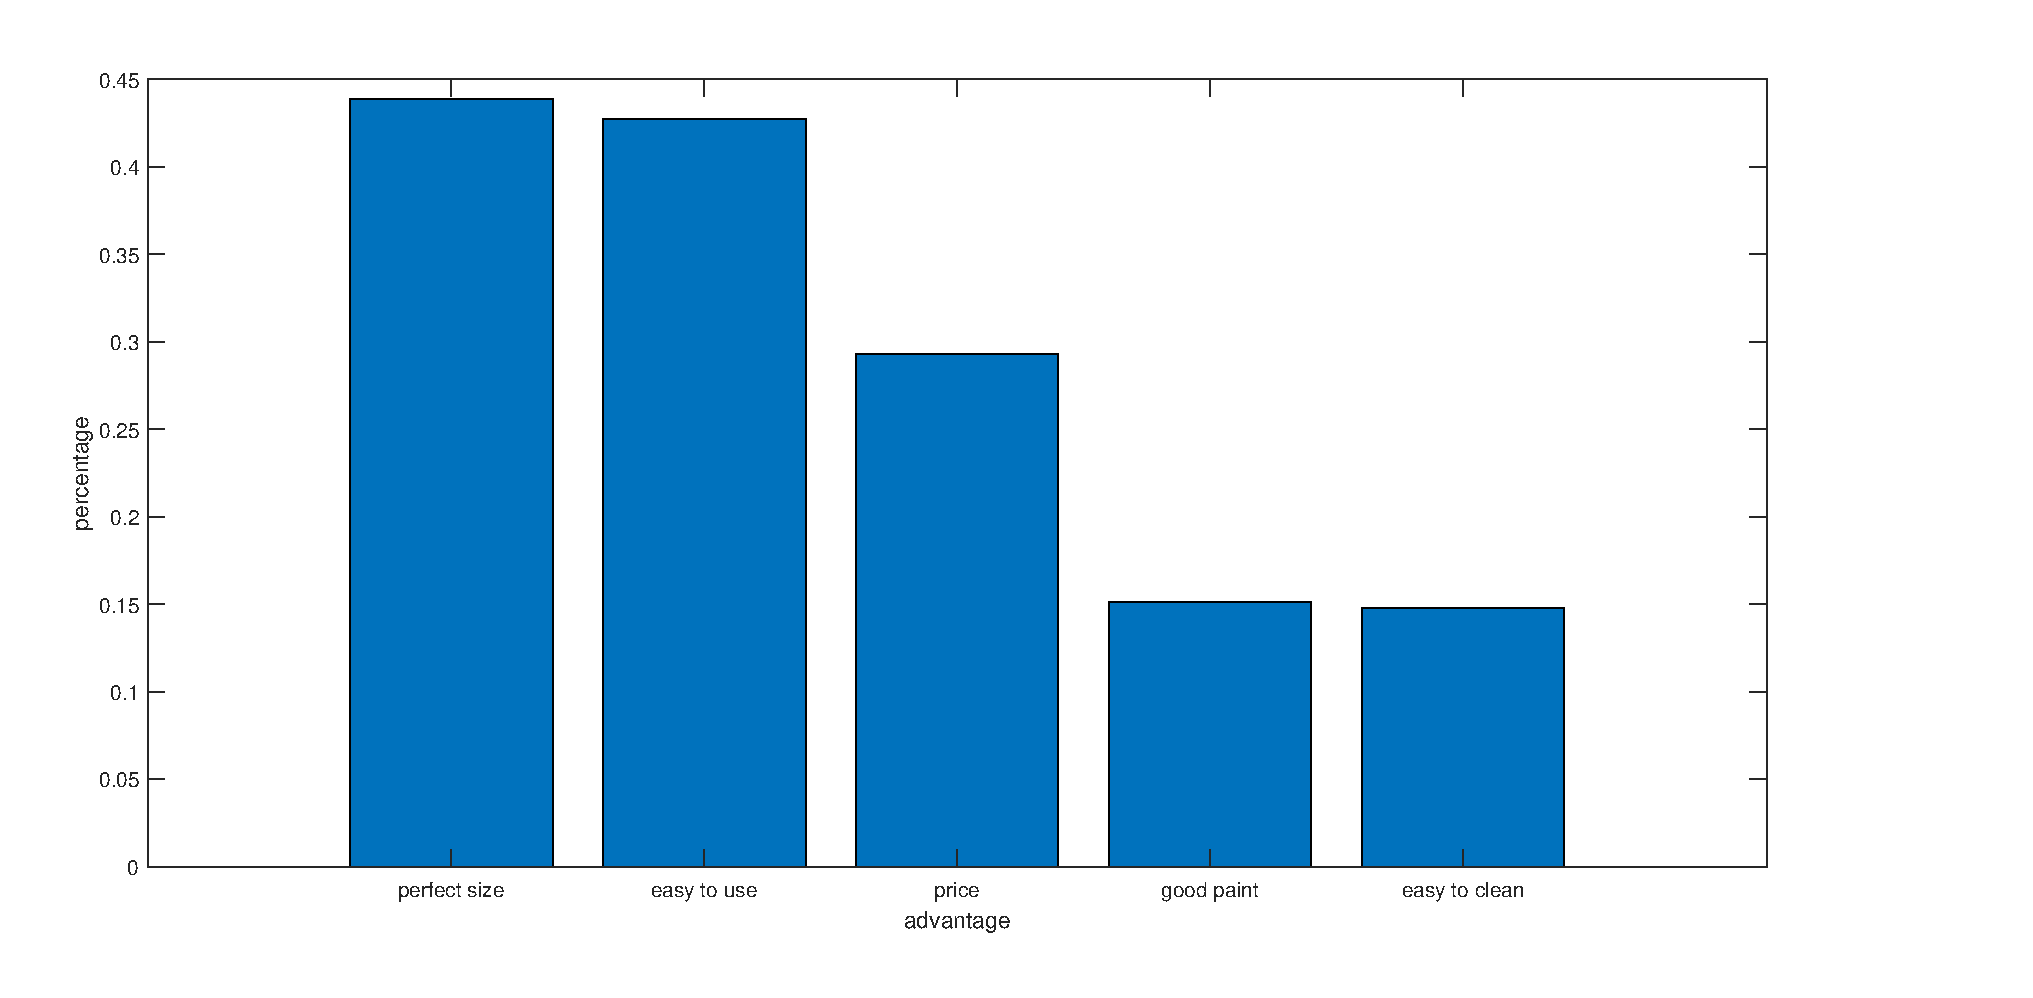
\includegraphics[width=9cm]{pacifier_advantage.eps}
			\caption{The proportion of reasons people like the baby pacifier\label{fig:1}}
		\end{minipage}
		\qquad
		\begin{minipage}[t]{0.5\textwidth}
			\centering
			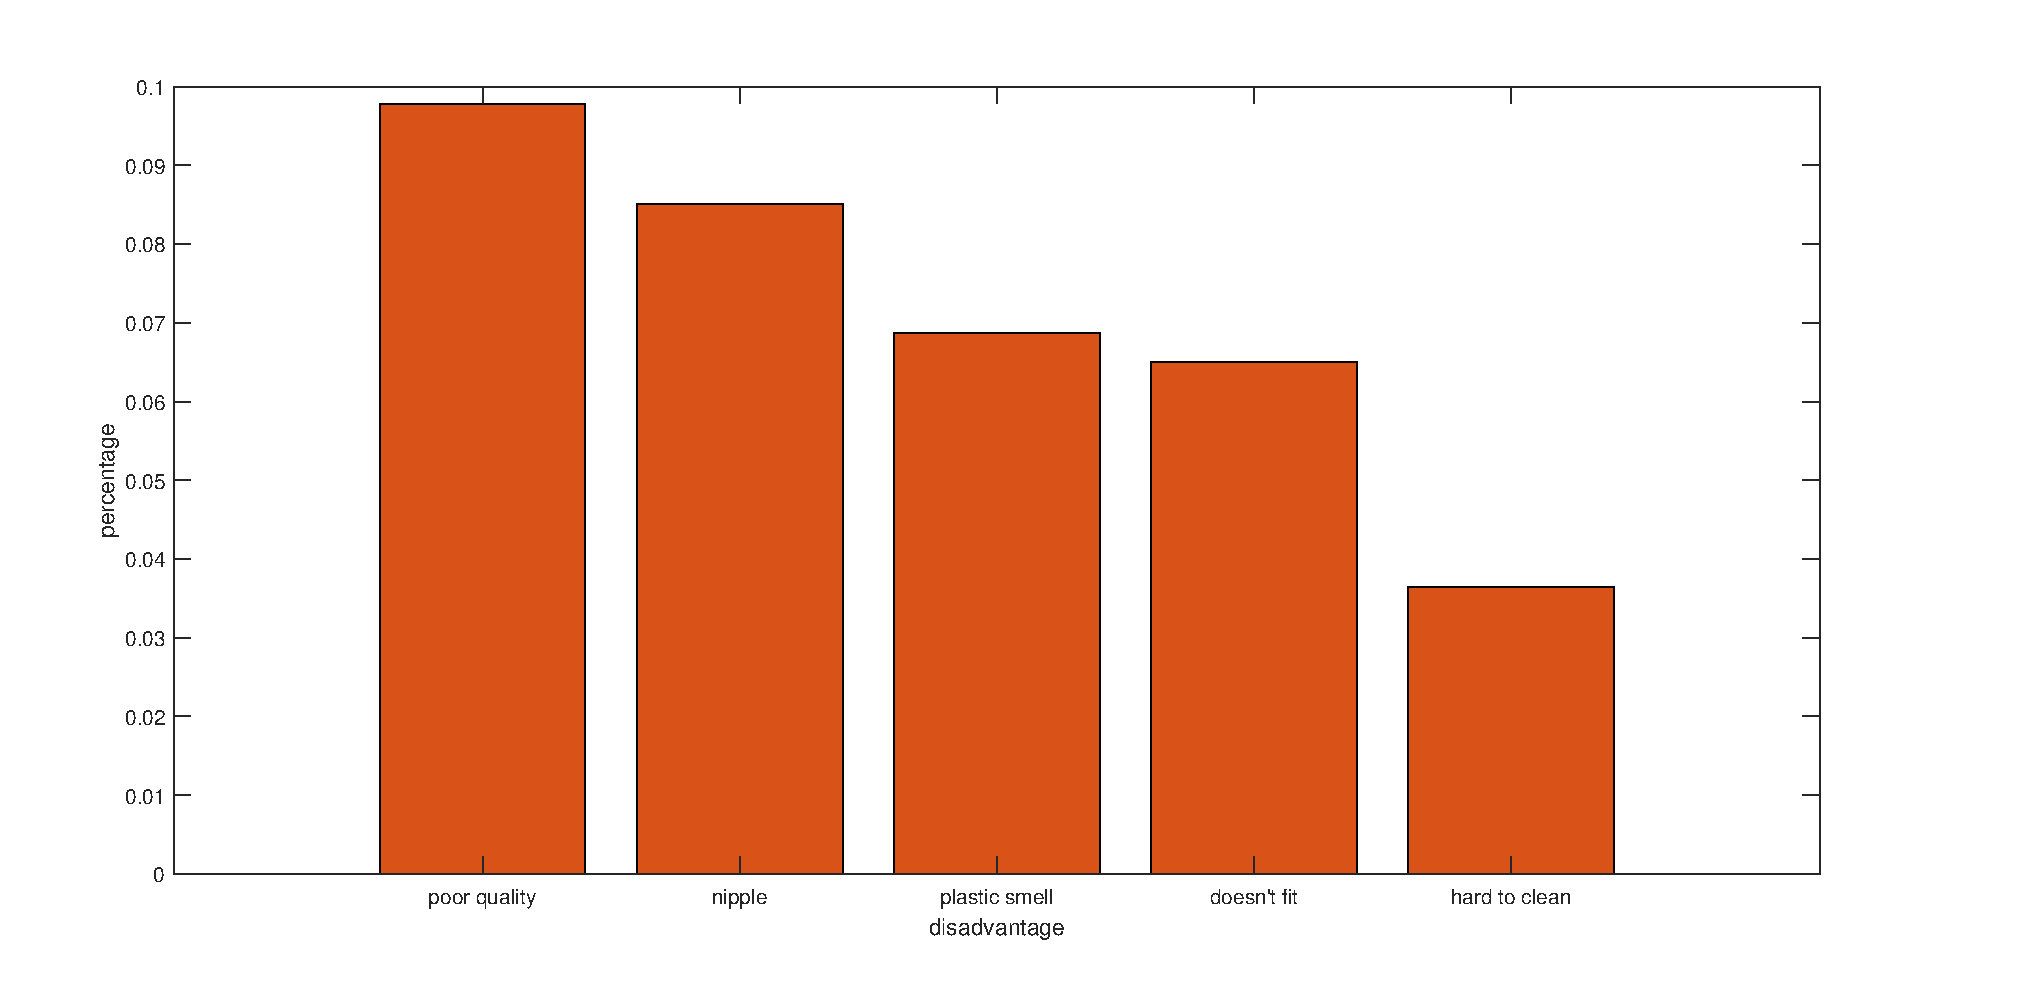
\includegraphics[width=9cm]{pacifier_disadvantage.eps}
			\caption{The proportion of reasons people dislike the baby pacifier\label{fig:2}}
		\end{minipage}
	\end{figure}
	
	As shown in the chart, ease of use is the most outstanding advantage of the product. About 17\% of high scoring customers mentioned this feature in their comments. After that is cute, quality, price and pacifier design.
	
	
	On the other hand, about 9.5\% of people who don't like the product complain about the poor quality. Although 4\% of people who like the product think that the nipple fits well with there baby's mouth, 7\%  think that the nipple leaks, or is too short and hard. Besides, people can't bear the plastic smell, which is an important reason why they don't like it. Furthermore, some parents think that baby pacifier doesn't fit well. At last, about 3\% of people find it hard to clean the pacifier, which makes them give low ratings.
	
	
	\subsubsection{Hair Dryer}
	\begin{figure}[H]
		\begin{minipage}[t]{0.5\textwidth}
			\centering
			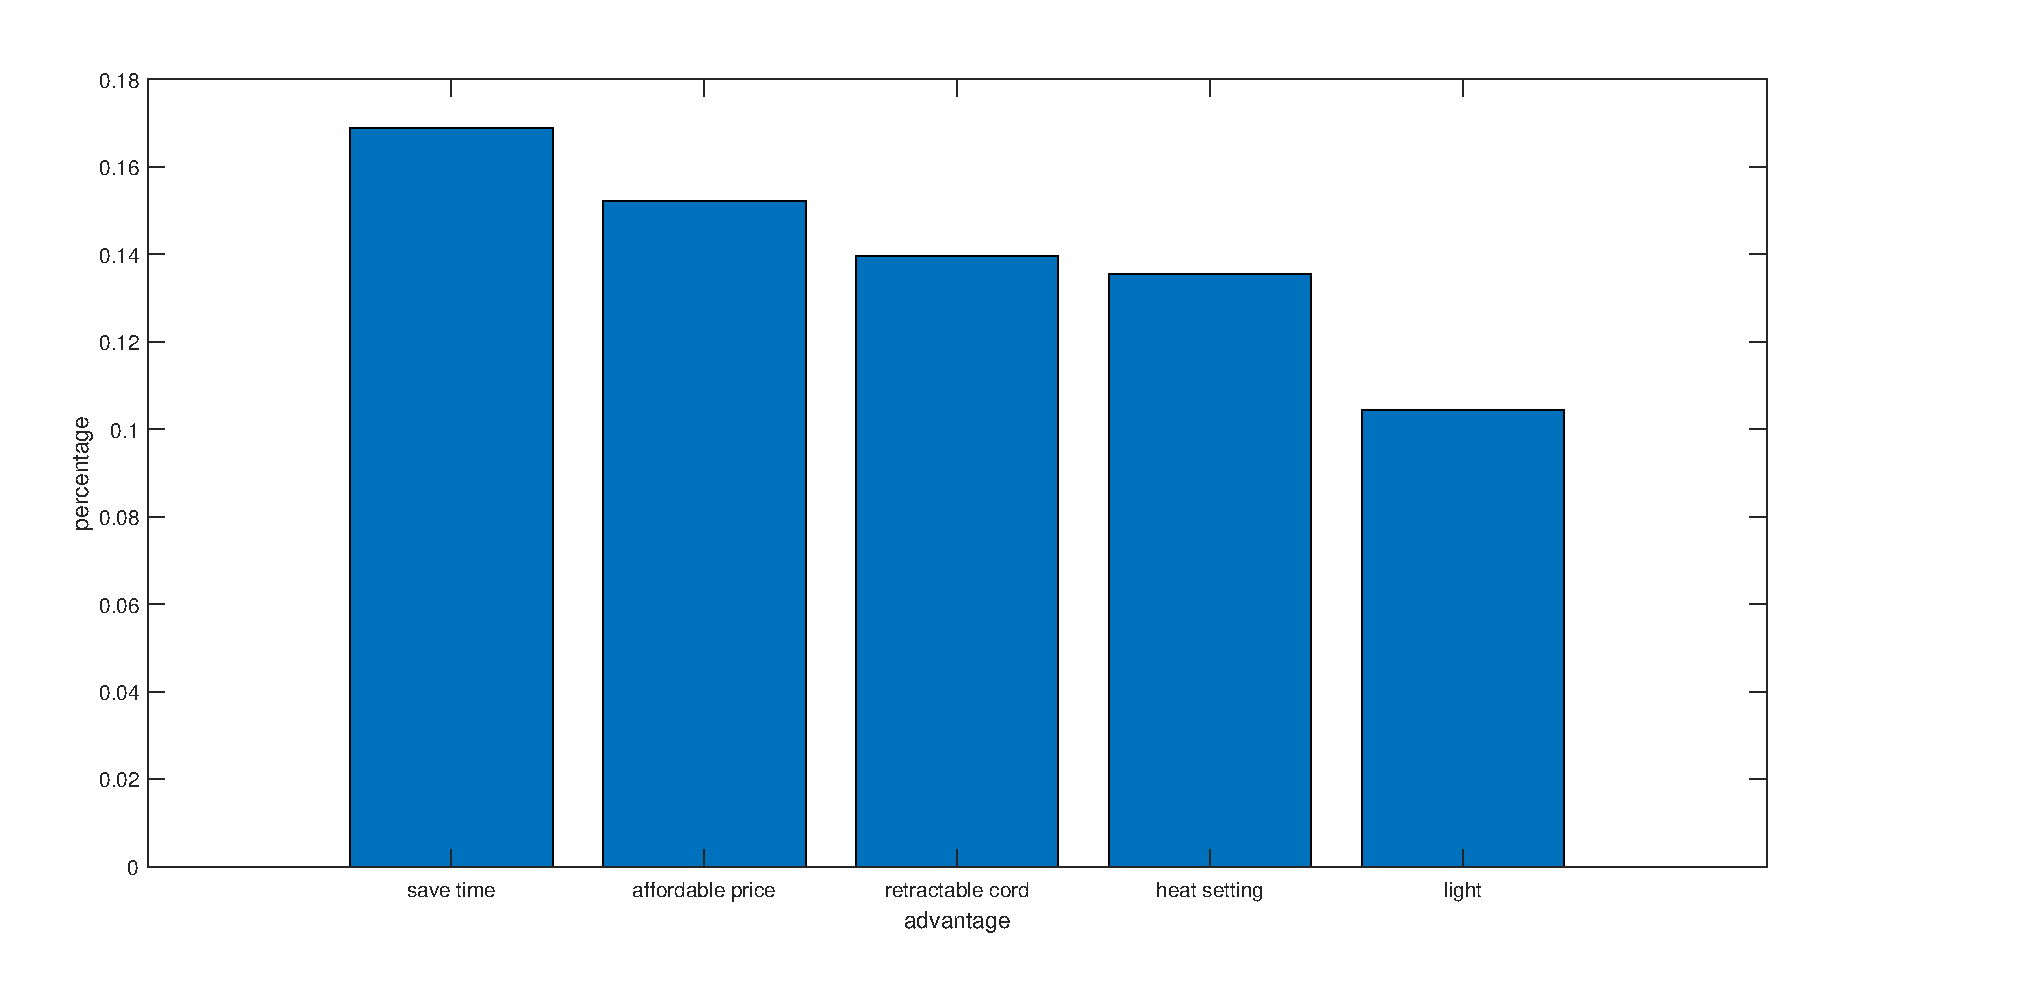
\includegraphics[width=9cm]{hair_dryer_advantage.eps}
			\caption{The proportion of reasons people like the hair dryer}
		\end{minipage}
		\qquad
		\begin{minipage}[t]{0.5\textwidth}
			\centering
			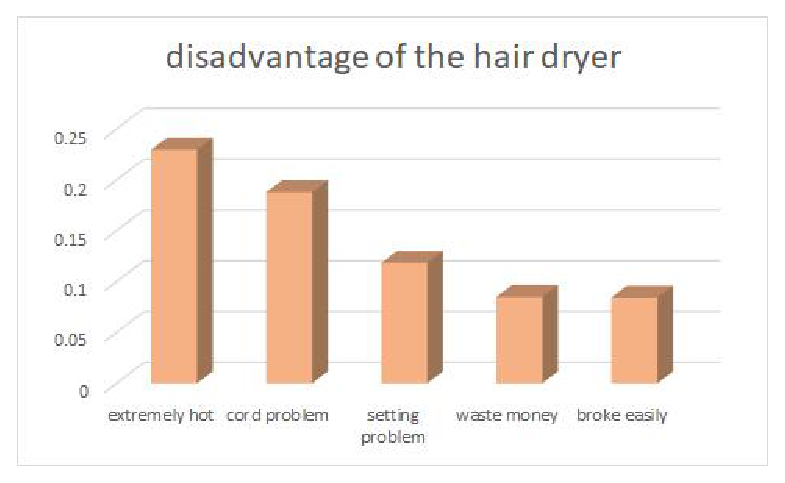
\includegraphics[width=9cm]{hair_dryer_disadvantage.eps}
			\caption{The proportion of reasons people dislike the hair dryer }
		\end{minipage}
	\end{figure}
	
	According to the figure,16\% of people think it saves their time, while 14\% were attracted by the affordable price.12\% think the retractable cord is good design. Besides, the hairdryer is light to carry, so 10\% of customers give a high rating. At last, the heating setting design is also attractive.
	
	From the figure, we can know that about 21\% of people can't stand the extreme hot of the hair dryer.17\% complained that the cord broke quickly.10\% find that the setting mode has some problem.7\% think buying the hairdryer is a waste of money, and the same percentage of people wrote that the hairdryer broke quickly.
	
	\subsubsection{Microwave Oven}
	\begin{figure}[H]
		\begin{minipage}[t]{0.5\textwidth}
			\centering
			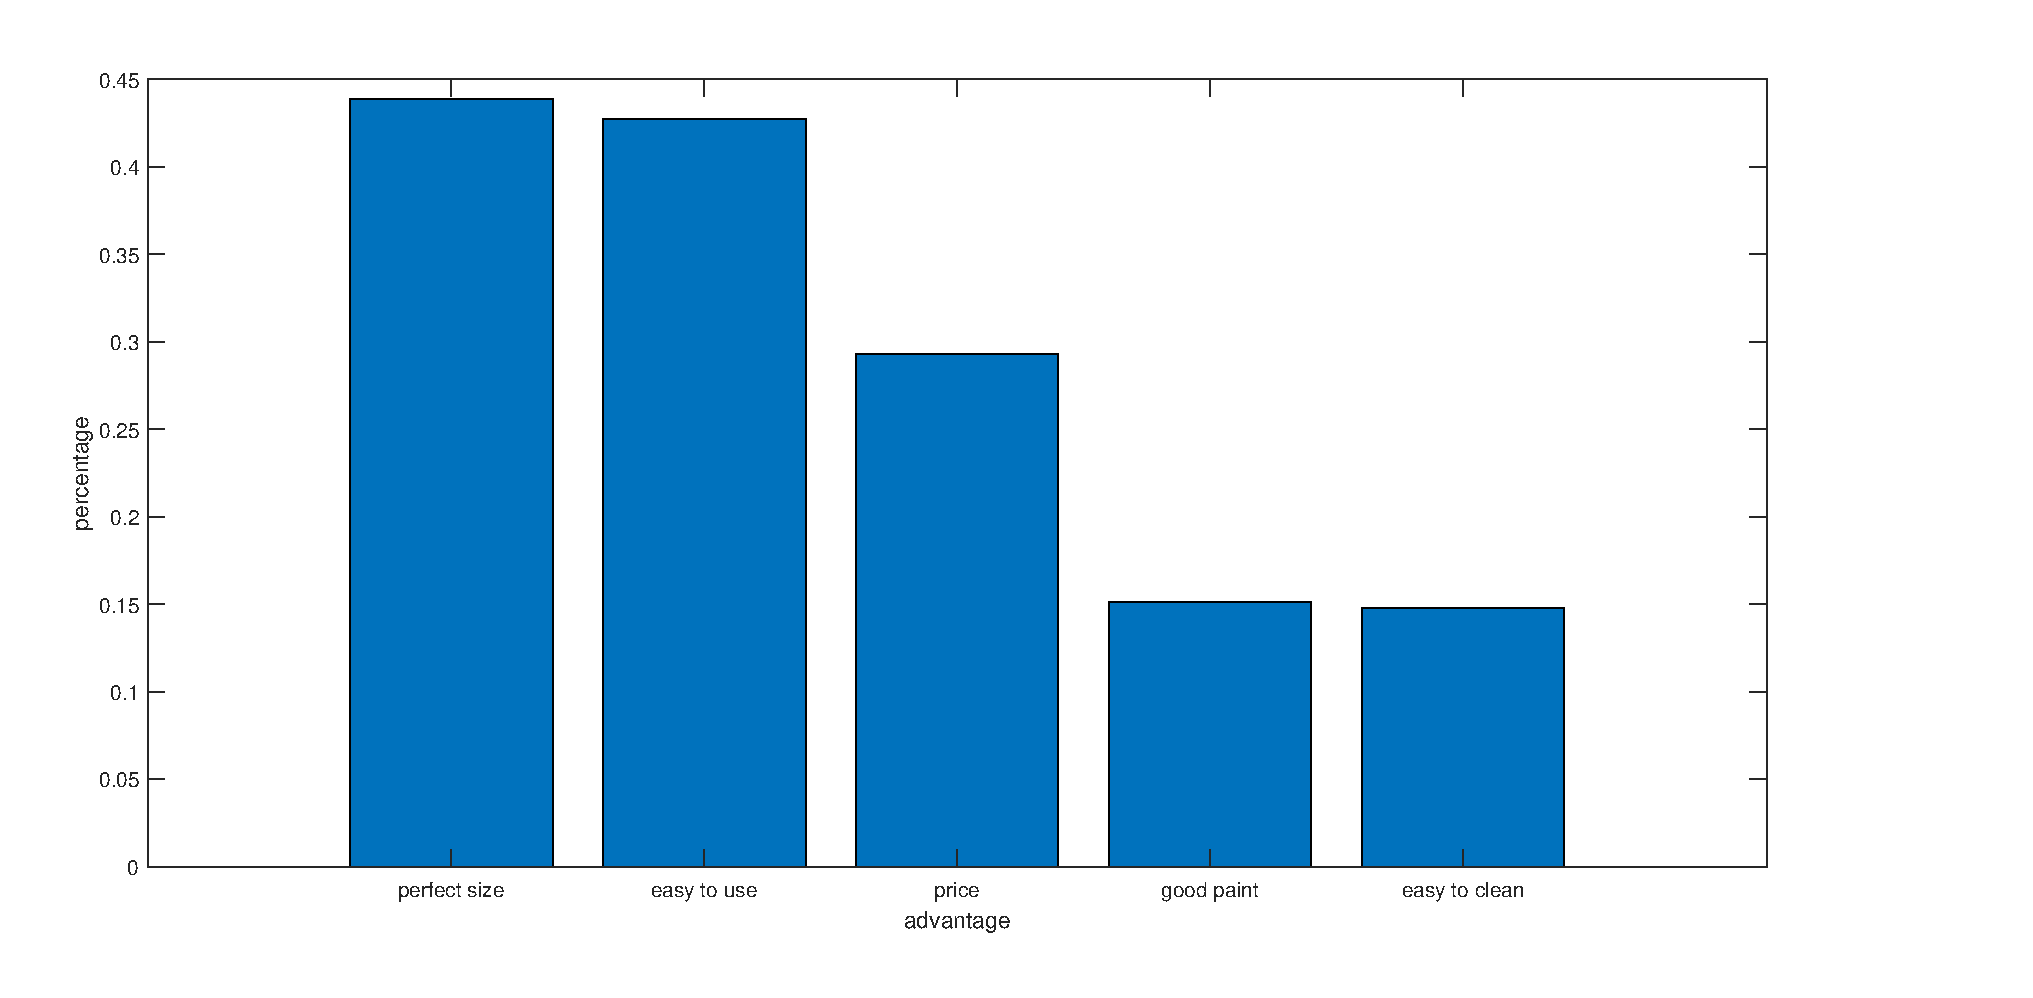
\includegraphics[width=9cm]{microwave_advantage.eps}
			\caption{The proportion of reasons people like the microwave oven\label{fig:1}}
		\end{minipage}
		\qquad
		\begin{minipage}[t]{0.5\textwidth}
			\centering
			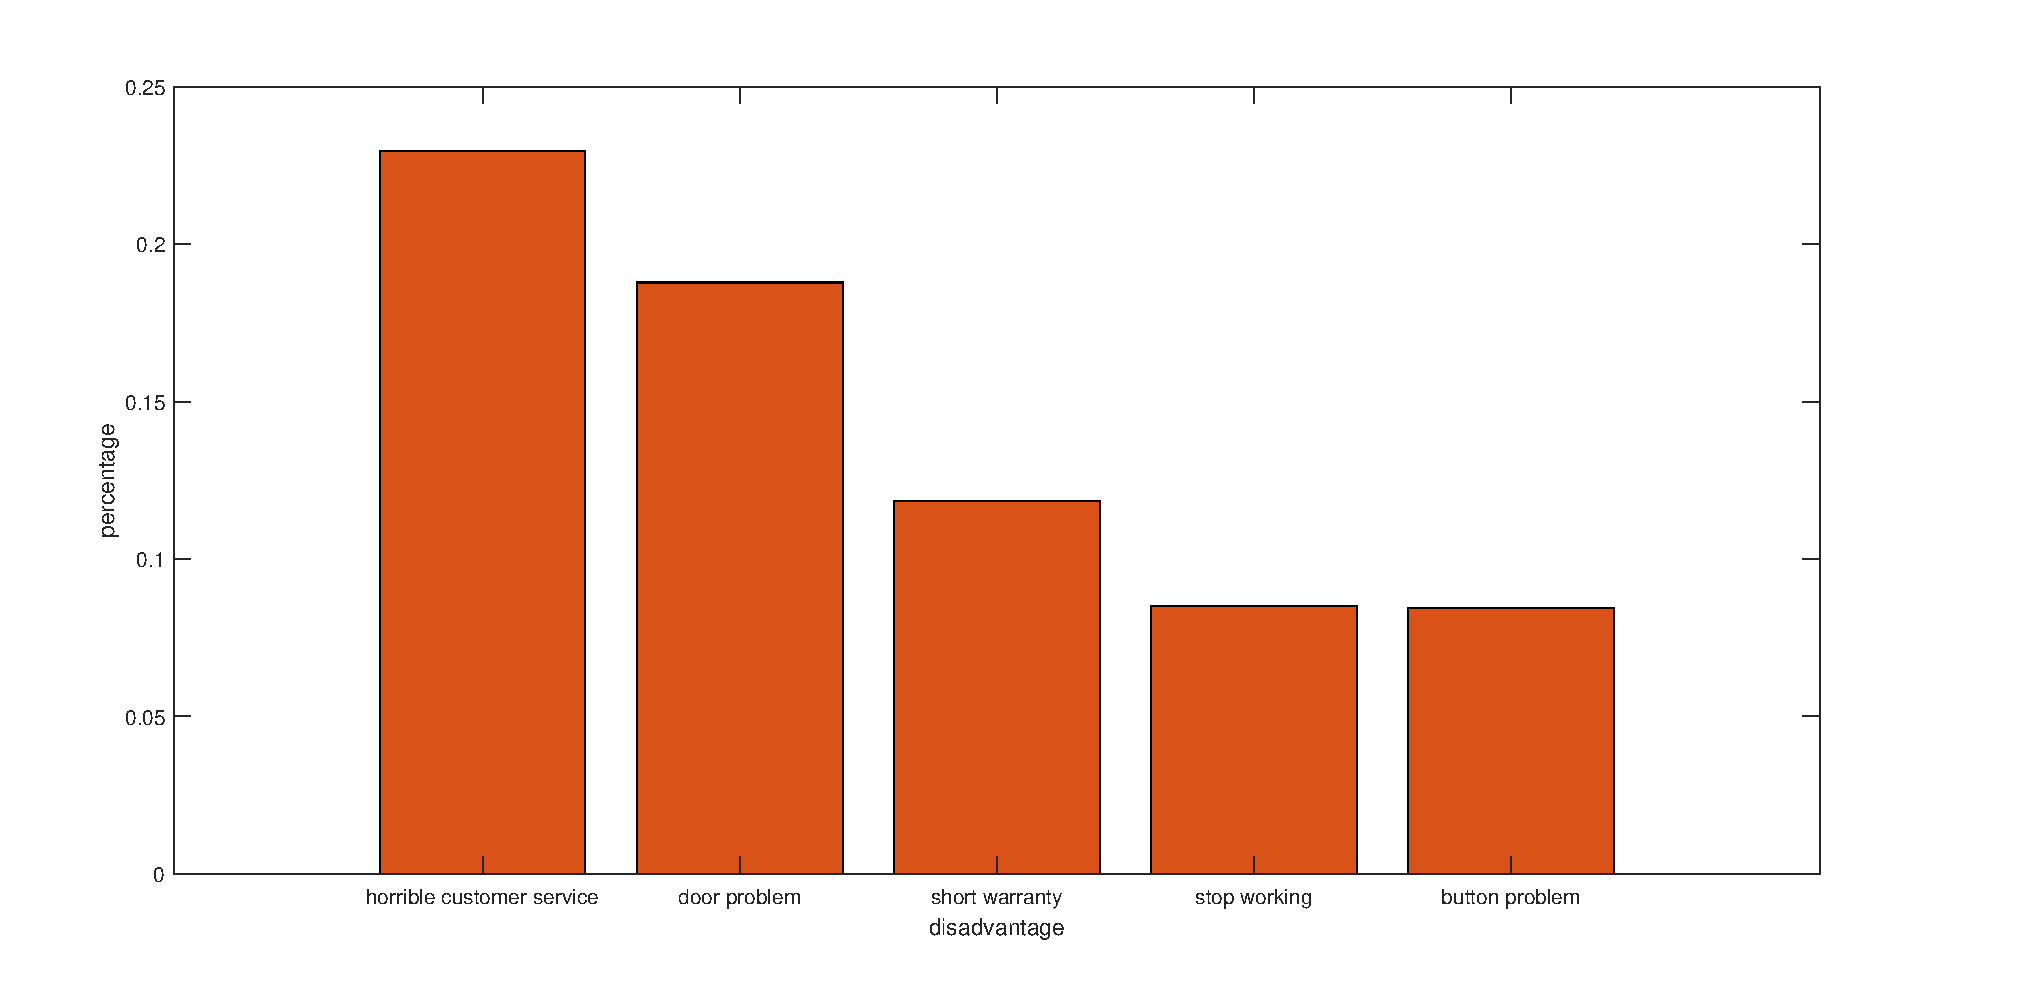
\includegraphics[width=9cm]{microwave_disadvantage.eps}
			\caption{The proportion of reasons people dislike the microwave oven\label{fig:2}}
		\end{minipage}
	\end{figure}
	
	About 35\% of customers love its size. They said they can put it anywhere in the kitchen and it fits well.21\% thinks it's easy to use.15\% people think that the price is fair.	6\% enjoy its paint. And some other people find the microwave oven easy to clean.
	
	However, problems still exist. Customers complain that the customer service is horrible. Besides, the door of the microwave oven has many problems. Furthermore,20\% think warranty time is too short. About 9\% of people said that their microwave ovens stop working or the button broke;
	
	
	
	\subsection{The Relationship between Quality Descriptors and Ratings}
	We choose 8 specific quality descriptors. And their frequency is shown in the table.
	\begin{table}[H]
		\centering
		\caption{The number of times the word was mentioned}
		\begin{tabular}{|c|c|c|c|c|c|c|c|c|}
			\hline 
			& love & perfect & nice & cute & disappointed & waste & bad & junk \\ 
			\hline 
			high rating & 8193 & 2591 & 2483 & 2435 & 165 & 65 & 339 & 20 \\ 
			\hline 
			low rating & 187 & 64 & 185 & 189 & 432 & 292 & 260 & 149 \\ 
			\hline 
		\end{tabular}
	\end{table}
	
	We calculated the probability of these words appearing in high rating reviews and low rating reviews, respectively.
	
	\begin{align}
	p(word\_in\_high\_rating)=\frac{\frac{num\_in\_high}{high\_num}}
	{\frac{num\_in\_high}{high\_num}+\frac{num\_in\_low}{low\_num}}
	\end{align}
	
	\begin{itemize}
		\item  $word\_in\_high\_rating$:Probability of words appearing in high scoring comments 
		\item	$num\_in\_high$ :The number of times words appear in high rated comments
		\item $num\_in\_low$ :The number of times words appear in low rated comments
		\item $high\_num$ :Number of high rated comments
		\item $low\_num$ :Number of low rated comments
	\end{itemize}
	
	
	\begin{figure}[H]
		\begin{minipage}[t]{1\textwidth}
			\centering
			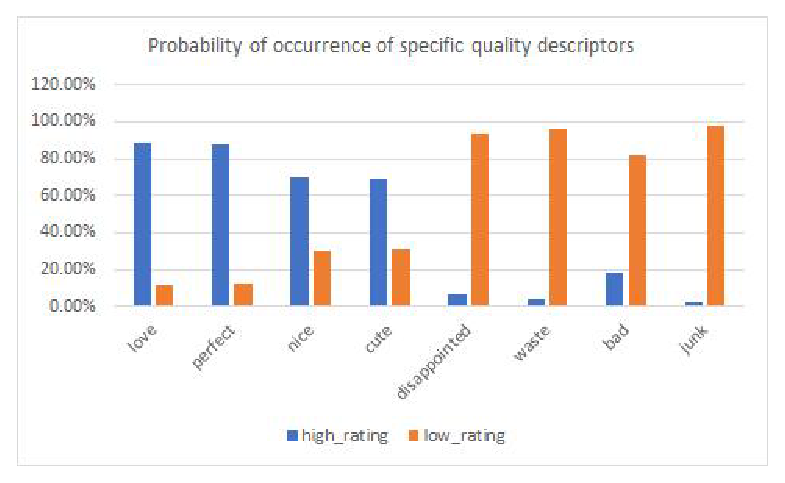
\includegraphics[width=19cm]{total.eps}
			\caption{probability the word appear in high/low rating comments\label{fig:1}}
		\end{minipage}
	\end{figure}
	
	As we can see, if the word 'love' or 'perfect' appears in the review, Users nearly have a 90\% chance to give high scores. On the contrary, if the word 'disappointed' is in the review, We can almost conclude that the user will give a low rating.
	
	So it is obvious that specific quality descriptors are strongly associated with rating levels.
	
	\subsection{Do specific star ratings incite more reviews? }
	\subsubsection{Theory}
	
	To analyze whether some specific star ratings lead to more reviews, we have analyzed the highest selling products for hair dryers, microwave ovens, and baby pacifiers. First, we counted the number of reviews per month for a certain product and the number of reviews per month for five ratings of the product and then used the correlation coefficient formula to calculate the correlation coefficient between the total number of reviews and a certain number of star ratings. The correlation coefficients corresponding to the scores are compared. When a certain correlation coefficient is large, the more the certain star ratings in a certain period, the more the user's comments will be. That is to say, the number of certain star ratings and the total number of star ratings are in a linear relationship. That way, we have every reason to believe that this rating will incite more reviews.
	
	\subsubsection{Data Processing}
	
	To calculate the correlation coefficient, we need to first calculate the covariance of these two data. Covariance can be easily calculated by the following equation:
	$$Cov(X,Y)=E[(X-E[X])(Y-E[Y])]$$
	
	Cov (X, Y) represents the covariance of X and Y, and E (X) represents the expectation of X.
	
	After getting the covariance, we used the following formula to calculate the correlation coefficient:
	$$r(X,Y)=\frac{Cov(X,Y)}{\sqrt{Var[X]Var[Y]}}$$
	
	Here r (X, Y) represents the correlation coefficient between X and Y, and Var [X] represents the variance of X.
	
	Here is the table of the correlation coefficient for every star rating:
	
	% Please add the following required packages to your document preamble:
	% \usepackage{graphicx}
	\begin{table}[H]
		\centering
		\caption{correlation coefficient for every star rating}
		\resizebox{120mm}{15mm}
		{%
			\begin{tabular}{|c|c|c|c|c|c|}
				\hline
				product    & star1 & star2 & star3 & star4 & star5 \\ \hline
				hair dryer & 0.68  & 0.46  & 0.69  & 0.85  & 0.97  \\ \hline
				microwave  & 0.58  & 0.38  & 0.6   & 0.57  & 0.72  \\ \hline
				pacifier   & 0.35  & 0.36  & 0.5   & 0.61  & 0.98  \\ \hline
			\end{tabular}%
		}
	\end{table}
	
	Here is the graph based on the above table:
	
	\begin{figure}[H]
		\small
		\centering
		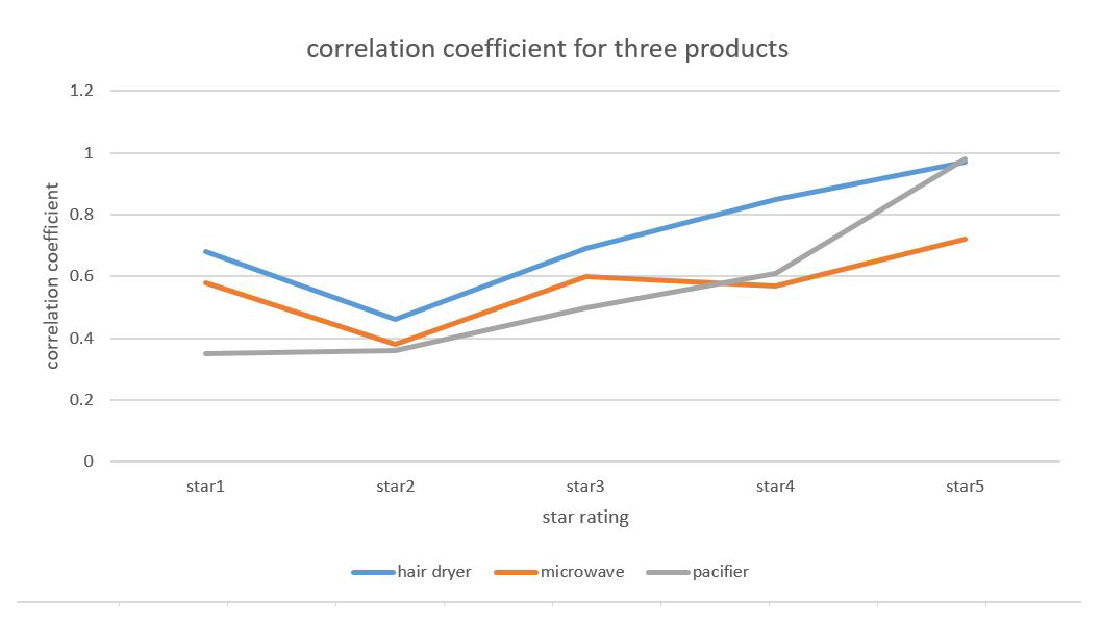
\includegraphics[width=15cm]{correlation_coefficient_incite.eps}
		\caption{correlation coefficient incite} \label{fig:correlation coefficient incite}
	\end{figure}
	
	\subsubsection{Conclusion}
	
	As can be seen from the above chart, the correlation coefficient with a star of 5 is the largest. This means that a 5-star rating will lead to more reviews.
	
	\subsection{Calculating the Score of Reviews Using DNN}
	The emotion analysis system is one of the most classical applications in natural language processing. We use the algorithm developed by Han Xiao and Yao Lu\cite{1} to map the degree of whether a customer likes or dislikes the product to the range of [0,1], to quantitatively reflect the attitude expressed by the comment.
	\subsubsection{Preprocessing}
	
	
	The original text data often has many parts that affect the final classification effect. This part of data or text needs to be cleaned at the beginning of text classification, otherwise, it will easily lead to the so-called "trash in, trash out" problem\cite{2}
	
	In addition to the steps of missing value processing, de-duplication processing and noise processing included in the data cleaning of general classification problems, we also clean up the following data:
	\begin{itemize}
		\item Non-text data: HTML tags, URL addresses, and other non-text content are often attached to the text, so it is necessary to clear this part of the content that is not helpful for classification.
		\item Meaningless text: Besides, the rest of the text, such as advertising content, copyright information, and personal signature, should also be filtered out, which should not be learned as features.
	\end{itemize}
	\subsubsection{Algorithm}
	In the algorithm, Dynamic Convolution Neural Network is used as the sentiment prediction algorithm. The network layers are set as follows:
	\begin{itemize}
		\item Embedding layer: set as the lowest layer, to get the vector representation for individual words to form the matrix representation of the sentence
		\item Convolutional Layer: extracts local features by performing 2d convolution on the sentence matrix
		\item K-max pooling layer: extracts kth strongest signals on a per-feature basis
		\item Folding layer: adds interaction among features by "folding" the input matrix
		\item Logistic regression layer: the final layer that predicts by assigning scores to each output label
	\end{itemize}
	
	
	\subsection{Verifying the Accuracy of Review-Based Ratings}
	In the previous subsection, we analyzed reviews using natural language processing and gave a score for each record. This subsection will verify the accuracy of the previously given score.
	
	We believe that the correlation coefficient between review-based ratings and star ratings can well reflect the accuracy of the analysis of the review. We calculated the total correlation coefficients of the three categories of products, and the correlation coefficients of high star rating (4-5) and low star rating (1-2). The results are as follows:
	
	
	
	\begin{table}[h]
		\begin{center} 
			\caption{the correlation coefficient between review-based ratings and star ratings}
			\begin{tabular}{|c|c|c|}
				\hline
				&                  & correlation coefficient \\ \hline
				\multirow{3}{*}{hair dryer}     & high star rating & 0.4201                  \\ \cline{2-3} 
				& low star rating  & 0.4934                  \\ \cline{2-3} 
				& all              & 0.5964                  \\ \hline
				\multirow{3}{*}{microwave oven} & high star rating & 0.3978                  \\ \cline{2-3} 
				& low star rating  & 0.5381                  \\ \cline{2-3} 
				& all              & 0.6753                  \\ \hline
				\multirow{3}{*}{baby pacifier}  & high star rating & 0.4372                  \\ \cline{2-3} 
				& low star rating  & 0.4557                  \\ \cline{2-3} 
				& all              & 0.5797                  \\ \hline
			\end{tabular}
		\end{center}
	\end{table}
	
	
	As can be seen from the table, review-based ratings are positively related to star rating satisfaction. In the case where the review-based score is relatively low, especially when the star rating is in the middle level, the correlation coefficient is relatively high. Overall our review-based ratings are acceptable.
	
	
	\subsection{User Evaluation}
	\subsubsection{Theory}
	To get a user evaluation of the top three hair dryers, microwave ovens, and baby pacifiers, we came up with the following measurement method. To make full use of reviews and ratings, we combined text-based ratings and star-based ratings, each giving different weights, and finally got a most informative measure. The formula is as follows:
	$$
	average\ rating = 0.8 \times star\_rating + text\_rating
	$$
	
	On top, star\_rating is between 1 and 5, text\_rating is between 0 and 1.
	\subsubsection{Data Processing}
	
	The statistical granularity is one month. Calculate the average scoring of all reviews each month, and draw a score-time chart. The calculations are done by Python. For the python code, see Appendix B.
	
	First of all, let's see the chart of the top three hair dryers\ (product\_id: B003V264WW, B0009XH6TG, B00132ZG3U):
	
	\begin{figure}[H]
		\small
		\centering
		\includegraphics[width=13cm]{hair_dryer_ave_rating2.eps}
		\caption{hair dryer average rating} \label{fig:hair dryer average rating}
	\end{figure}
	
	Combining the above figure, we find that the average score curves of these three products are very similar. In the early stages, product ratings fluctuated greatly because there were fewer customers. For example, the product B0009XH6TG (red line) has fluctuated between 1 and 5 stars in the early stage, the product B003V264WW (blue line) has fluctuated between 3 stars and 5 stars in the early stage, and the product B00132ZG3U (green line) has also fluctuated between 3 stars and 5 stars. In the later period, the scores of the three products stabilized at about 4 points, and the fluctuations did not exceed 0.5 points. It can be seen that the ratings of these three products in the later period are similar.
	
	Secondly, here is the chart of the top three microwave ovens\    (product\_id: B0055UBB40, B0058CLNBU, B0052G14E8):
	
	\begin{figure}[H]
		\small
		\centering
		\includegraphics[width=13cm]{microwave_ave_rating2.eps}
		\caption{microwave oven average rating} \label{fig:micorwave average rating}
	\end{figure}
	
	    This picture is not different from the above picture, because the microwave oven has fewer reviews, the average rating fluctuates greatly. First of all, the product B0055UBB40 (red line) has been fluctuating between one star and three stars. Secondly, the product B0058CLNBU (blue line) has been fluctuating between one star and five stars, and the blue line has been almost above the red line. The final product B0052G14E8 (green line) fluctuated between one star and five stars in the early stage and stabilized at about four stars in the later stage. It can be seen that the market feedback of product B0058CLNBU (blue line) and product B0052G14E8 (green line) is better than product B0055UBB40 (red line).
	
	Finally, the chart of the top three baby pacifiers is as follow:\ (product\_id: B003CK3LLDI, B0028IDXDS, B0045I6IA4):
	\begin{figure}[H]
		\small
		\centering
		\includegraphics[width=13cm]{pacifier_ave_rating2.eps}
		\caption{baby pacifier average rating} \label{fig:pacifier average rating}
	\end{figure}
	This picture is very similar to the picture about the hair dryer, both of which fluctuate in the early stage and stabilize in the later stage. In the later period, the three products were stable between four stars and 4.5 stars. In this regard, market feedback is better than hair dryers.
	
	\subsection{Comprehensive Evaluation}
	\subsubsection{Theory}
	In the previous subsection, we gave a measurement scheme based on the user star rating and review analysis only, which focuses more on user evaluation. But sometimes sales, helpful votes and whether a buyer is a vine can also affect the measurement of a product. Therefore, we designed another general evaluation formula:
	
	$$review\_score=(text\_rating\times4-2)\times(10+helpful\_votes-(total\_votes-helpful\_votes))$$
	
	$$rating\_score=star\_rating\times10\times(1+isvine)$$
	
	$$total\_score=max(0,\frac{review\_score+rating\_score\times4}{100})$$
	
	On top, star\_rating is between 1 and 5, text\_rating is between 0 and 1.
	
	\subsubsection{Data Processing}
	We sum the total score of all the reviews every month and select the top three products to draw a line chart. The results are as follows:
	
	\begin{figure}[H]
		\small
		\centering
		\includegraphics[width=13cm]{hair_dryer_total_score2.eps}
		\caption{hair dryer total score} \label{fig:hair dryer total score}
	\end{figure}
	
	Combined with the previous chart, we can see that for the hair dryer, the three products have the same rating, and there are some differences in sales. This is also reflected in the total score: the overall rating of the product B003V264WW (black line) is slightly better than the other two products. But in general, all three products are very competitive. If you want to take the lead in this product category, you must have a unique advantage.
	
	\begin{figure}[H]
		\small
		\centering
		\includegraphics[width=13cm]{microwave_total_score2.eps}
		\caption{microwave oven total score} \label{fig:microwave total score}
	\end{figure}
	
	For microwave ovens, the difference is obvious. Product B0052G14E8 (black line) has always maintained a good score; product B0058CLNBU (blue line) has always had a low score; product B0055UBB4O (red line) has increased rapidly after a period of low scores. This may be because product B0055UBB4O (the red line) made up for the shortcomings in the sales process, resulting in a large increase in sales. It can be seen that if some fatal flaws are avoided, the company can easily occupy a good microwave oven market share.
	
	\begin{figure}[H]
		\small
		\centering
		\includegraphics[width=13cm]{pacifier_total_score2.eps}
		\caption{baby pacifier total score} \label{fig:pacifier total score}
	\end{figure}
	
	The market competition for baby pacifiers is also fierce, with three products taking the lead alternately. However, we have noticed that the total scores of these products have been declining recently. So if you want to join the market for baby pacifiers, it's important to seize this opportunity.
	
	In general, we believe that the formula for calculating a total score can reflect the sales of goods very well. By comparing the total scores with other similar products or with the total score of a certain period before, the company can clearly understand the sales situation and adjust the sales strategy.
	
	
	\section{Conclusion}
	
	In this paper, we used NLP, correlation coefficients, and word frequency statistics to analyze the sales of existing products on the market and user feedback.
	
	The analysis of the following three products is based on the three evaluation indicators above: sales volume, average score, and total score. The average rating combines text-based ratings and star ratings, reflecting user feedback. The total score combines multiple indicators, which are proportional to the market sales, text-based ratings, star ratings, and the number of useful votes, so it can accurately reflect the market response of the product.
	
	The competition in the hair dryer market is very fierce, and the top three products with similar sales ratios and ratings are similar. Among them, the product B003V264WW has the shortest history, but the average score has remained at a high level, and the market share and total score have advanced rapidly. This shows that this product has its unique advantages and has more references for Sunshine Company. According to word frequency surveys of high-scoring reviews, these words often appear: save time, save money, heat controllability, and lightness. These advantages should be valued by Sunshine. But at the same time avoid the disadvantages of easy damage.
	
	The competition in the microwave oven market is not so fierce. Recently, two products (B0052G14E8 and B0055UBB40) accounted for a large proportion, and the product B0052G14E8 has only entered the market for two years. This shows that the microwave oven market has great potential. Sunshine can invest more. But the product B0052G14E8's average score and total score are both relatively high, which indicates that if Sunshine's newly launched products have unique competitiveness, it may occupy a large market in a short period. According to word frequency analysis, the following advantages should be valued: proper size, ease of use, cheap price, good paint, easy cleaning, and robustness.
	
	Finally, the top three products in the baby pacifier market all have a long history. This shows that users have high requirements for the quality of baby pacifiers, and they are very sticky. Of course, this is also well understood. Parents will not easily change brands for the sake of their children's health. If Sunshine wants to enter this market, then the quality requirements must be given special attention. According to word frequency analysis, a good product should have such advantages: easy to use, cute in appearance, high quality, reasonable price, comfortable to use, easy to clean, and tasteless.
	
	Based on the calculation of the correlation coefficient, we find that 5-star reviews are more likely to incite more reviews. This also means that if a product has good feedback when it first enters the market, then other users are more likely to pay.
	
	\newpage
	
	\section{Letter}
	\begin{flushleft}
		Dear Director:
	\end{flushleft}
	\paragraph{}
	I write to you on behalf of the MCM team 2010225. As soon as we know that you are going to launch and sell the products, we have analyzed the historical sales data of these three types of products. I hope it can help you to develop your sales strategy.
	
	    First of all, we analyzed the sales volume of the three products. 
	In general, hair dryers and baby pacifiers sell more than microwave ovens. The details of the three products are as follows:
	
	For hair dryer, some new products have a rapid growth in sales in a short period, surpassing many old products with slow growth in sales. Besides, the total sales volume of the hair dryer has increased rapidly in recent years. So if your product quality is excellent, you will have great development opportunities. 
	
	The sales volume of microwave ovens fluctuates greatly. Some products are not selling well all the time, but many new products sell well as soon as they come into the market. This may be because consumers of microwave ovens prefer the new features of the product.
	
	The overall increase in sales of baby pacifiers may be related to the increase in the number of newborns, which is good for you. But the best selling goods have a long sale time. This may be because people prefer to choose safe and reliable old brands with large sales volume and high praise. So you should pay more attention to quality and make good reputation.
	
	Then we have statistical research on customer reviews. Through the research of some words that often appear in the reviews, we have summed up the five most praised and questioned features of the three types of products, hoping to help you to summarize the experience and lessons.
	
	For baby pacifier, safety and quality are the main concerns of customers. It's worth mentioning that many customers complain that many products in the past have a plastic smell. If you make an improvement, it will certainly help you win more customers. For hair dryer, people pay more attention to the comfort and price of use, and we can consider developing affordable and convenient products. For the microwave oven, people are very concerned about their size and after-sales service. Because the microwave oven is a long-term product, so you need to pay attention to after-sales service. If you can, extending the warranty will also win you more customers.
	\paragraph{}
	Finally, we set a comprehensive value for you to evaluate your sales situation in the future, which integrates the customer's comments, scores, vote on the comments, whether the customer is vine and other factors. You can use it to make a comprehensive assessment of your sales situation and compare it with previous products to help you sell products better.
	
	Hope our advice will help you.
	\flushleft
	Sincerely yours
	\flushleft
	MCM 2020 Team 2010225
	
	\newpage
	
	\begin{thebibliography}{99}
		\bibitem{1} http://xiaohan2012.github.io/twitter-sent-dnn/
		\bibitem{2} Hu M , Liu B . Mining and summarizing customer reviews[C]// Proceedings of the Tenth ACM SIGKDD International Conference on Knowledge Discovery and Data Mining, Seattle, Washington, USA, August 22-25, 2004. ACM, 2004.
		
	\end{thebibliography}
	
	\newpage
	
	\begin{appendices}
		\section{}
		\textcolor[rgb]{0.98,0.00,0.00}{\textbf{Input python source:}}
		\lstinputlisting[language=python]{./code/count_word_frequency.py}
		\newpage
		\section{}
		\textcolor[rgb]{0.98,0.00,0.00}{\textbf{Input python source:}}
		\lstinputlisting[language=python]{./code/average_rating.py}
	\end{appendices}
\end{document}

%%
%% This work consists of these files mcmthesis.dtx,
%%                                   figures/ and
%%                                   code/,
%% and the derived files             mcmthesis.cls,
%%                                   mcmthesis-demo.tex,
%%                                   README,
%%                                   LICENSE,
%%                                   mcmthesis.pdf and
%%                                   mcmthesis-demo.pdf.
%%
%% End of file `mcmthesis-demo.tex'.

